%!TEX program = xelatex
\documentclass[10pt,twocolumn,letterpaper]{article}

\usepackage{cvpr}
\usepackage{times}
\usepackage{epsfig}
\usepackage{graphicx}
\usepackage{tabularx}
\usepackage{amsmath}
\usepackage{amssymb}
\usepackage{amsthm}
\usepackage{algorithm2e}
\usepackage{authblk}


% Include other packages here, before hyperref.

% If you comment hyperref and then uncomment it, you should delete
% egpaper.aux before re-running latex.  (Or just hit 'q' on the first latex
% run, let it finish, and you should be clear).
\usepackage[pagebackref=true,breaklinks=true,letterpaper=true,colorlinks,bookmarks=false]{hyperref}

\usepackage{fontspec}

\cvprfinalcopy % *** Uncomment this line for the final submission

\def\cvprPaperID{407} % *** Enter the CVPR Paper ID here
\def\httilde{\mbox{\tt\raisebox{-.5ex}{\symbol{126}}}}

\def\vec{\mathbf}
\def\mat{\mathbf}

\newtheorem{lemma}{Lemma}
\newtheorem{theorem}{Theorem}
\newtheorem{proposition}{Proposition}

% Pages are numbered in submission mode, and unnumbered in camera-ready
\ifcvprfinal\pagestyle{empty}\fi
\begin{document}

\RestyleAlgo{boxruled}

%%%%%%%%% TITLE
\title{Learning From Massive Noisy Labeled Data for Image Classification}

\author[1]{Tong Xiao}
\author[2]{Tian Xia}
\author[2]{Yi Yang}
\author[2]{Chang Huang}
\author[1]{Xiaogang Wang}

\affil[1]{The Chinese University of Hong Kong}
\affil[2]{Baidu Research}

\renewcommand\Authands{, and }

% For a paper whose authors are all at the same institution,
% omit the following lines up until the closing ``}''.
% Additional authors and addresses can be added with ``\and'',
% just like the second author.
% To save space, use either the email address or home page, not both

\maketitle
%\thispagestyle{empty}

%%%%%%%%% ABSTRACT
\begin{abstract}
Large-scale supervised datasets are crucial to train convolutional neural networks (CNNs) for various computer vision problems. However, obtaining a massive amount of well labeled data is usually very expensive and time consuming. In this paper, we introduce a general framework to train CNNs with only a limited number of clean labels and millions of easily obtained noisy labels. We describe label noises with a probabilistic graphical model and further integrate it into an end-to-end deep learning system. To demonstrate the effectiveness of our approach, we collect a large-scale clothing classification dataset with both noisy and clean labels. Experiments on this dataset show that our model can better detect and correct the wrong labels, which benefits the training of underlying CNNs.
\end{abstract}

%%%%%%%%% BODY TEXT
\section{Introduction} % (fold)
\label{sec:introduction}

Deep learning with a massive amount of supervised training data has recently shown very impressive improvement on multiple image recognition challenges including image classification~\cite{krizhevsky2012imagenet}, attribute learning~\cite{zhang2013panda}, and scene classification~\cite{farabet2013learning}. While state-of-the-art results have been continuously reported~\cite{zeiler2013visualizing,simonyan2014very,szegedy2014going}, all these methods require reliable annotations from millions of images~\cite{deng2009imagenet} which are often expensive and time-consuming to obtain~\cite{deng2009imagenet}, preventing deep models from being quickly trained on new image recognition problems. Thus it is necessary to develop new efficient labeling and training frameworks for deep learning.

One possible solution is to automatically collect large amount of annotations from the Internet web images~\cite{gong2014multiview} (i.e. extracting tags from the surrounding texts or keywords from search engines) and directly use them as ground truth to train deep models. Unfortunately, these labels are extremely unreliable due to various types of noise (i.e. labeling mistakes from annotators or computing errors from extraction algorithms). Many works have shown that these noisy labels could adversely impact the classification accuracy of the induced classifiers~\cite{zhu2004class,nettleton2010study,pechenizkiy2006class}. Various label noise-robust algorithms are developed but experiments show that performances of classifiers inferred by robust algorithms are still affected by label noise~\cite{bartlett2006convexity,teng2001comparison}. Other data cleansing algorithms are proposed~\cite{barandela2000decontamination,brodley2011identifying,miranda2009use}, but these approaches are difficult in distinguishing informative hard examples from harmful mislabeled ones.

\begin{figure}[t]
\begin{center}
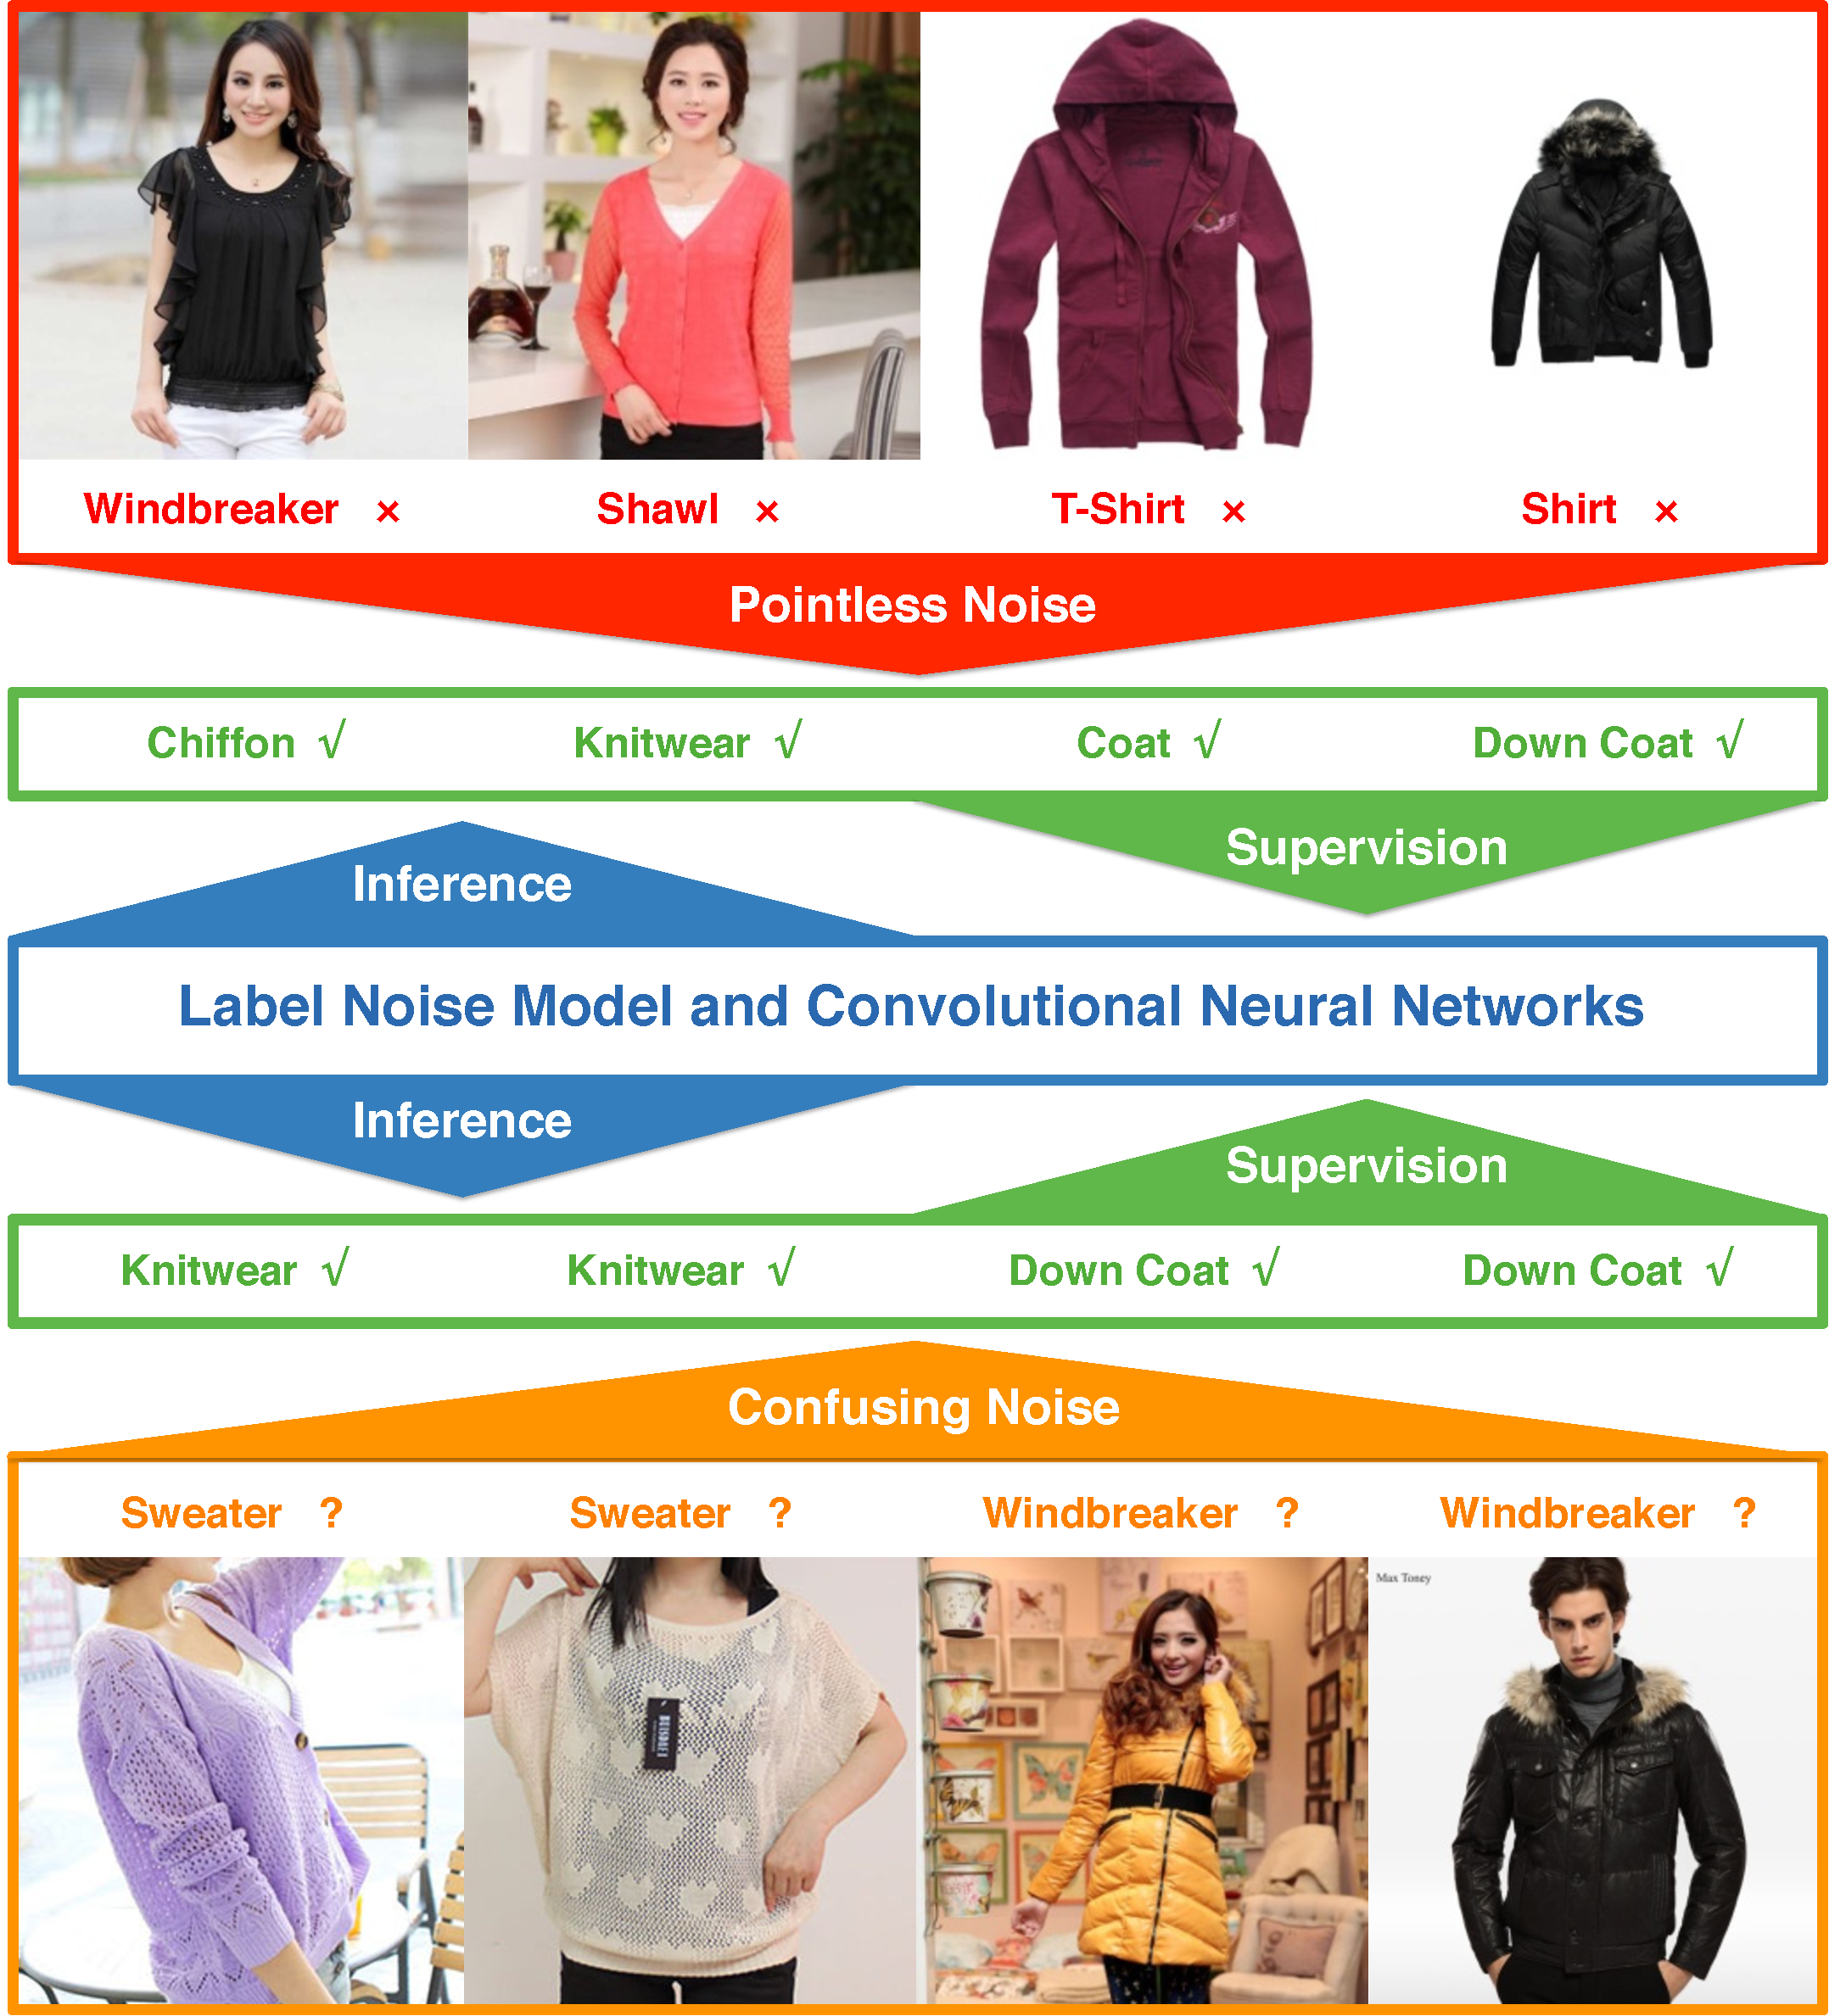
\includegraphics[width=0.95\linewidth]{figure/overview.pdf}
\end{center}
\caption{Overview of our approach. Labels of web images often suffer from different types of noise. A label noise model is proposed to detect and correct the wrong labels. The corrected labels are used to train underlying CNNs.}
\label{fig:overview}
\end{figure}

Although annotating all the data is costly, it is often easy to obtain a small amount of clean labels. Based on the observation of transferability of deep neural networks, people initialize parameters with a model pretrained on a larger yet related dataset~\cite{krizhevsky2012imagenet}, and then finetune on the smaller dataset of specific tasks~\cite{oquab2013learning,azizpour2014generic,donahue2013decaf}. Such methods may better avoid overfitting and utilize the relationships between the two datasets. However, we find that training a CNN from scratch with limited clean labels and massive noisy labels is better than finetuning it only on clean labels. Other approaches address the problem as semi-supervised learning where noisy labels are discarded~\cite{zhu2002learning}. These algorithms usually suffer from model complexity thus cannot be applied on large-scale datasets. Therefore, it is inevitable to develop a better way of using huge amount of noisy labeled data.

Our goal is to build an end-to-end deep learning system that is capable of training with both limited clean labels and massive noisy labels more effectively. Figure~\ref{fig:overview} shows the framework of our approach. We collect $1,000,000$ clothing images from online shopping websites. Each image is automatically assigned with a noisy label according to the keywords in its surrounding text. We manually refine $72,409$ image labels, which constitute a clean sub-dataset. All the data are then used to train CNNs, while the major challenge is to identify and correct wrong labels during the training process.

To cope with this challenge, we extend CNNs with a novel probabilistic model, which infers the true labels and uses them to supervise the training of the network. Our work is inspired by~\cite{sukhbaatar2014learning}, which modified a CNN by inserting a linear layer on top of the softmax layer to map clean labels to noisy labels. However,~\cite{sukhbaatar2014learning} assumed noisy labels were conditionally independent with input images given clean labels. By examining our collected dataset, we find that this assumption is too strong to fit real-world data well. For example, in Figure~\ref{fig:noise_cluster}, all the images should belong to ``Hoodie''. The top five are correct while the bottom five are either mislabeled as ``Windbreaker'' or ``Jacket''. It shows that images tend to be mislabeled may share similar visual patterns. This is because different sellers have their own bias on different categories, thus they may provide wrong keywords for many similar clothes. Based on these observations, we introduce two types of label noise:
\begin{itemize}
\item \textbf{Confusing noise} makes the noisy label reasonably wrong. It usually occurs when the image content is confusing (\eg, the samples with ``?'' in Figure~\ref{fig:overview}).
\item \textbf{Pure random noise} makes the noisy label totally wrong. It is often caused by either the mismatch between an image and its surrounding text, or false conversion from the text to label (\eg, the samples with ``$\times$'' in Figure~\ref{fig:overview}).
\end{itemize}

The proposed probabilistic model builds the relations among images, noisy labels, ground truth labels, and noise types, where the latter two are treated as latent variables. We use the Expectation-Maximization (EM) algorithm to solve the problem and integrate it into the training process of CNNs. Experiments on the collected dataset show that our model can better detect and correct the wrong labels.

Our contribution comes from three aspects. First, we study the cause of noisy labels in real-world data and describe it with a novel probabilistic model. Second, we integrate the model into a deep learning framework to help detect and correct wrong labels. We study different training strategies to make the CNNs learn from better supervisions. Finally, we collect a large-scale clothing dataset with both noisy and clean labels, which will be released for academic use.

\begin{figure}[t]
\begin{center}
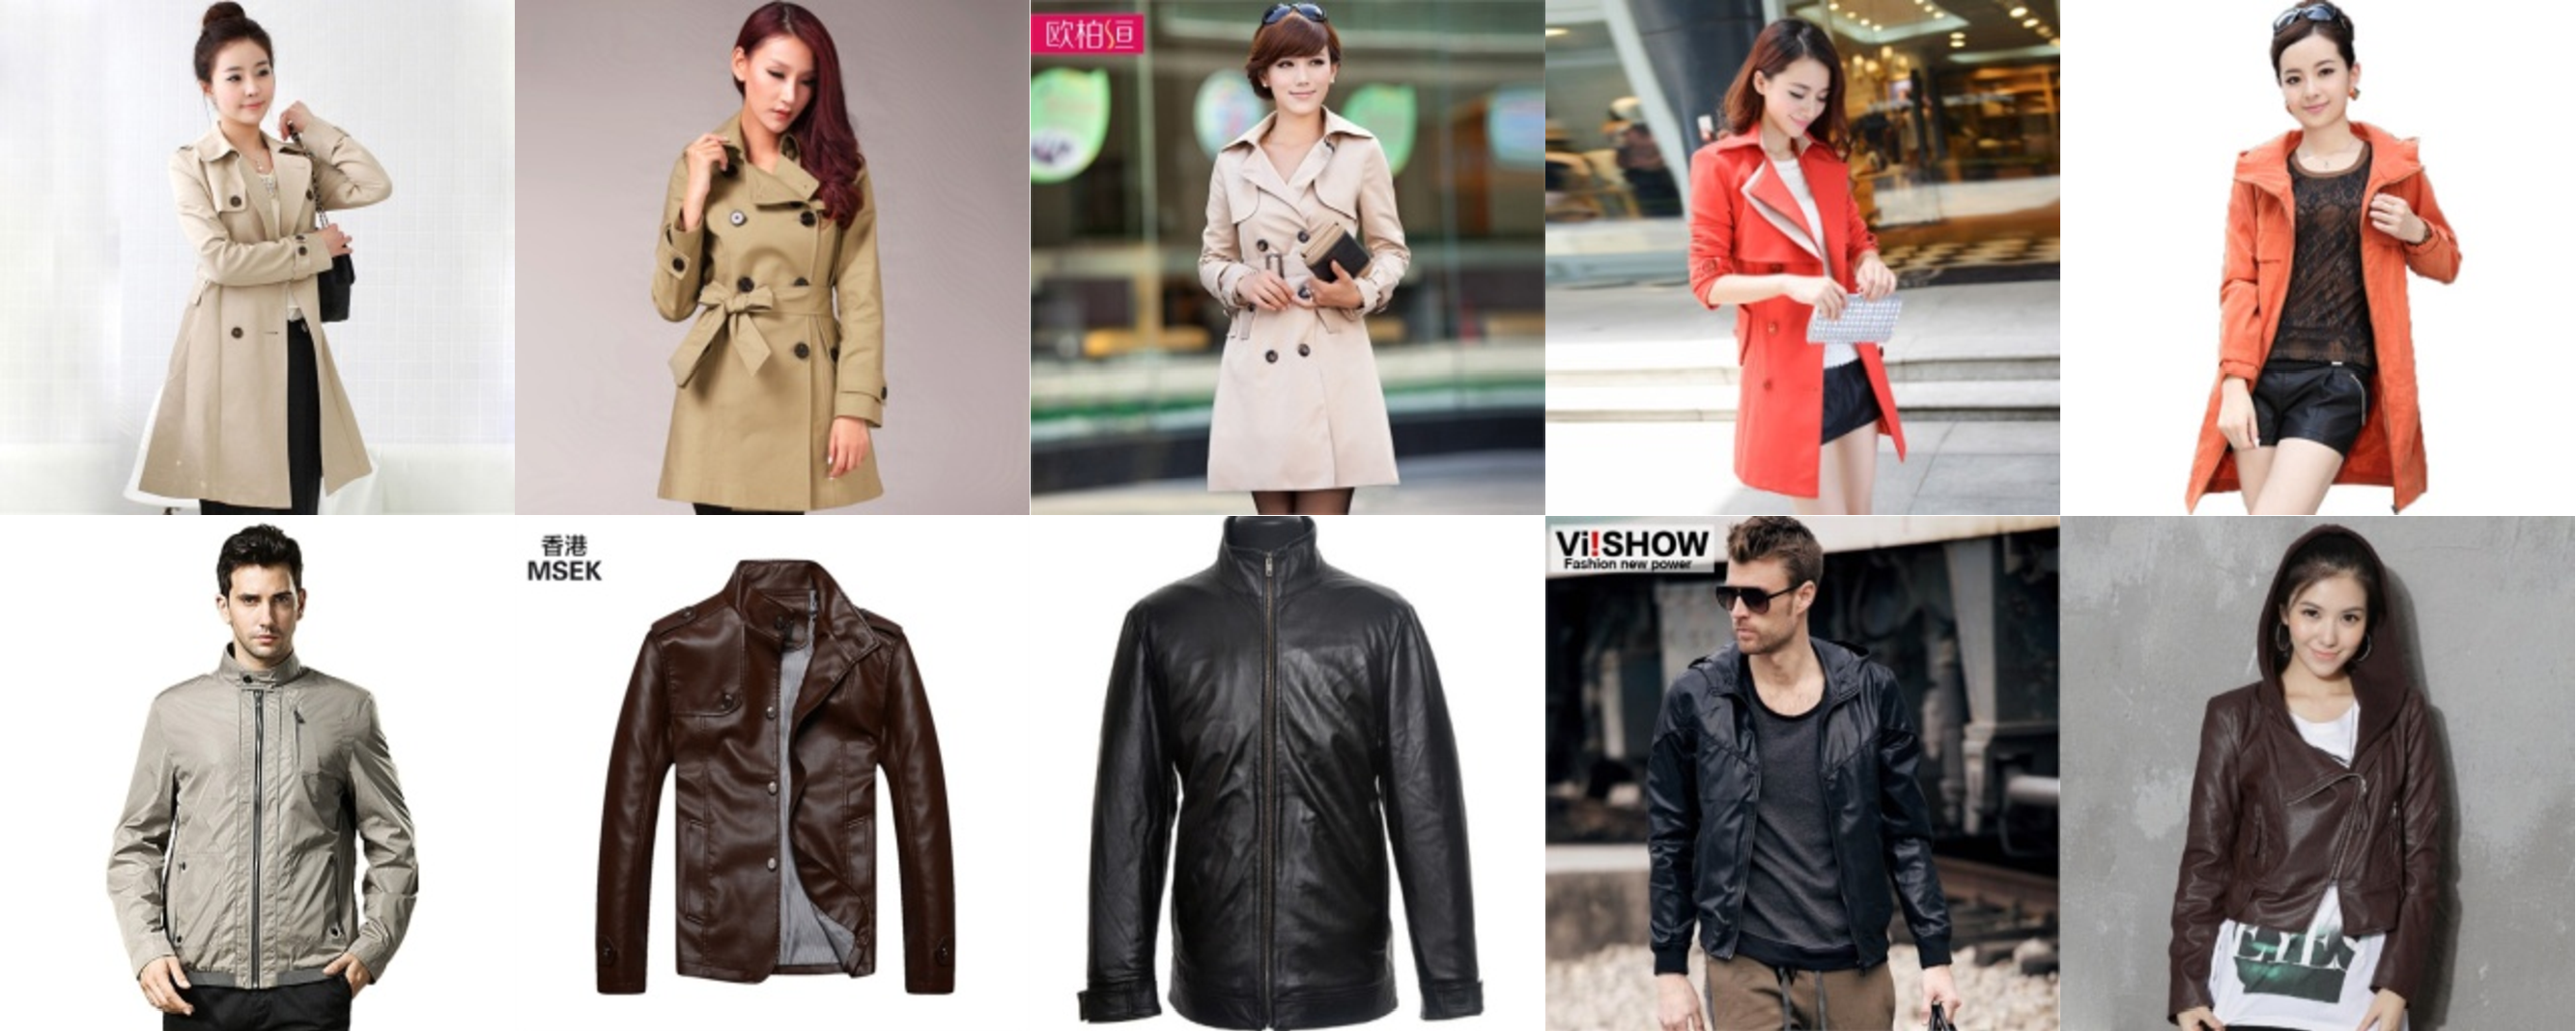
\includegraphics[width=1.0\linewidth]{figure/noise_cluster.pdf}
\end{center}
\caption{Images tend to be mislabeled often share similar visual patterns.}
\label{fig:noise_cluster}
\end{figure}
% section introduction (end)

\section{Related Work} % (fold)
\label{sec:related_work}
For most of the related works including the effect of label noises, taxonomy of label noises, robust algorithms and noise cleaning algorithms for learning with noisy data, we refer to~\cite{frenay2013classification} for a comprehensive review. 

{\bf Direct learning with noisy labels:} Many works have shown that label noise can adversely impact the classification accuracy of induced classifiers~\cite{zhu2004class}. To better handle label noise, some approaches rely on training classifiers with label noise-robust algorithms~\cite{beigman2009learning,manwani2013noise}. However, Bartlett \etal~\cite{bartlett2006convexity} proved that most of the loss functions are not completely robust to label noise. Experiments in~\cite{teng2001comparison} showed that the classifiers inferred by label noise-robust algorithms are still affected by label noise. These methods seem to be adequate only when label noise can be safely managed by overfitting avoidance~\cite{frenay2013classification}. On the other hand, some label noise cleansing methods were proposed to remove or correct mislabeled instances~\cite{barandela2000decontamination,brodley2011identifying,miranda2009use}, but these approaches were difficult in distinguishing informative hard examples from harmful mislabeled ones. Thus they might remove too many instances and the overcleansing could reduce the performances of classifiers~\cite{matic1992computer}.

{\bf Semi-supervised learning:} Apart from direct learning with label noise, some semi-supervised learning algorithms were developed to utilize weakly labeled or even unlabeled data. The Label Propagation method~\cite{zhu2002learning} explicitly used ground truths of well labeled data to classify unlabeled samples. However, it suffered from computing pairwise distance, which has quadratic complexity with the number of samples thus cannot be applied on large-scale datasets. Weston \etal~\cite{weston2012deep} proposed to embed a pairwise loss in the middle layer of a deep neural network, which benefits the learning of discriminative features. But they needed extra information about whether a pair of unlabeled images belong to the same class, which cannot be obtained in our problem.

{\bf Transfer learning:} The success of CNNs lies in their capability of learning rich and hierarchical image features. However, the model parameters cannot be properly learned when training data is not enough. Researchers proposed to conquer this problem by first initializing CNN parameters with a model pretrained on a larger yet related dataset, and then finetuning it on the smaller dataset of specific task~\cite{krizhevsky2012imagenet, oquab2013learning, azizpour2014generic,donahue2013decaf}. Nevertheless, this transfer learning scheme could be suboptimal when the two tasks are just loosely related. In our case of clothing classification, we find that training a CNN from scratch with limited clean labels and massive noisy labels is better than finetuning it only on the clean labels.

{\bf Noise modeling with deep learning:} Various methods have been proposed to handle label noise in different problem settings, but there are very few works about deep learning from noisy labels~\cite{mnih2012learning, larsen1998design, sukhbaatar2014learning}. Mnih and Hinton~\cite{mnih2012learning} built a simple noise model for aerial images but only considered binary classification. Larsen \etal~\cite{larsen1998design} assumed label noises are independent from true class labels which is a simple and special case. Sukhbaatar \etal~\cite{sukhbaatar2014learning} generalized from them by considering multi-class classification and modeling class dependent noise, but they assumed the noise was conditionally independent with the image content, ignoring the hardness of labeling images of different confusing levels. Our work can be viewed as a generalization of~\cite{sukhbaatar2014learning,natarajan2013learning} and our model is flexible enough to not only class dependent noise but also input dependent noise.
% section related_work (end)

\section{Label Noise Model} % (fold)
\label{sec:label_noise_model}
We target on learning a classifier from a set of images with noisy labels. To be specific, we have a noisy labeled dataset $\mathcal{D}_{\eta}=\left\{\left(\vec{x}^{(1)}, \tilde{y}^{(1)}\right), \dots, \left(\vec{x}^{(N)}, \tilde{y}^{(N)}\right)\right\}$ with $n$-th image $\vec{x}^{(n)}$ and its corresponding noisy label $\tilde{y}^{(n)} \in \{1,\dots,L\}$, where $L$ is the number of classes. We describe how the noisy label is generated by using a probabilistic graphical model shown in Figure~\ref{fig:noise_pgm}.

\begin{figure}[h!]
\begin{center}
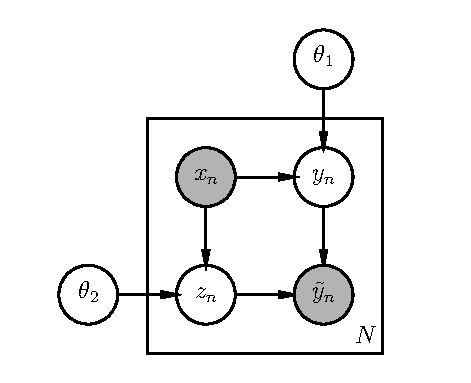
\includegraphics[width=0.5\linewidth]{figure/pgm.pdf}
\end{center}
\caption{Probabilistic graphical model of label noise}
\label{fig:noise_pgm}
\end{figure}

Despite the observed image $\vec{x}$ and the noisy label $\tilde{\vec{y}}$, we exploit two discrete latent variables --- $\vec{y}$ and $\vec{z}$ --- to represent the true label and the label noise type, respectively. Both $\tilde{\vec{y}}$ and $\vec{y}$ are $L$-dimensional binary random variables in 1-of-$L$ fashion, \ie, only one element is equal to 1 while others are all 0.

The label noise type $\vec{z}$ is an 1-of-3 binary random variable. It is associated with three different semantic meanings:
\begin{enumerate}
    \item The label is noise free, \ie, $\tilde{\vec{y}}$ should be equal to $\vec{y}$
    \item The label suffers from a pure random noise, \ie, $\tilde{\vec{y}}$ can take any possible value other than $\vec{y}$
    \item The label suffers from a confusing noise, \ie, $\tilde{\vec{y}}$ can take several values that are confusing with $\vec{y}$
\end{enumerate}

Following this assignment rule, we define the conditional probability of the noisy label as
\begin{equation} \label{eq:likelihood}
    p(\tilde{\vec{y}}|\vec{y},\vec{z}) = \begin{cases}
        \tilde{\vec{y}}^{T}\mat{I}\vec{y} & \text{if } \vec{z}_1 = 1 \\
        \frac{1}{L-1}\tilde{\vec{y}}^{T}(\mat{U} - \mat{I})\vec{y} & \text{if } \vec{z}_2 = 1 \\
        \tilde{\vec{y}}^{T}\mat{C}\vec{y} & \text{if } \vec{z}_3 = 1
    \end{cases}
\end{equation}
where $\mat{I}$ is the identity matrix, $\mat{U}$ is the unit matrix (all the elements are ones), $\mat{C}$ is a sparse stochastic matrix with $\mathrm{tr}(\mat{C})=0$ and $\mat{C}_{ij}$ denotes the confusion probability between classes $i$ and $j$. Then we can derive from Figure~\ref{fig:noise_pgm} the joint distribution of $\tilde{\vec{y}}, \vec{y}$ and $\vec{z}$ conditioning on $\vec{x}$:
\begin{equation} \label{eq:joint_distribution}
  p(\tilde{\vec{y}}, \vec{y}, \vec{z} | \vec{x}) = p(\tilde{\vec{y}} | \vec{y}, \vec{z}) p(\vec{y} | \vec{x}) p(\vec{z} | \vec{x})
\end{equation}

While the class label probability distribution $p(\vec{y} | \vec{x})$ is comprehensible, the semantic meaning of $p(\vec{z} | \vec{x})$ needs extra clarification: it represents how confusing the image content is. Specific to our clothing classification problem, $p(\vec{z} | \vec{x})$ can be affected by different factors, including background clutter, image resolution, the style and material of the clothes. Some examples are shown in Figure~\ref{fig:compare_noise_level}.

\begin{figure}[t]
\begin{center}
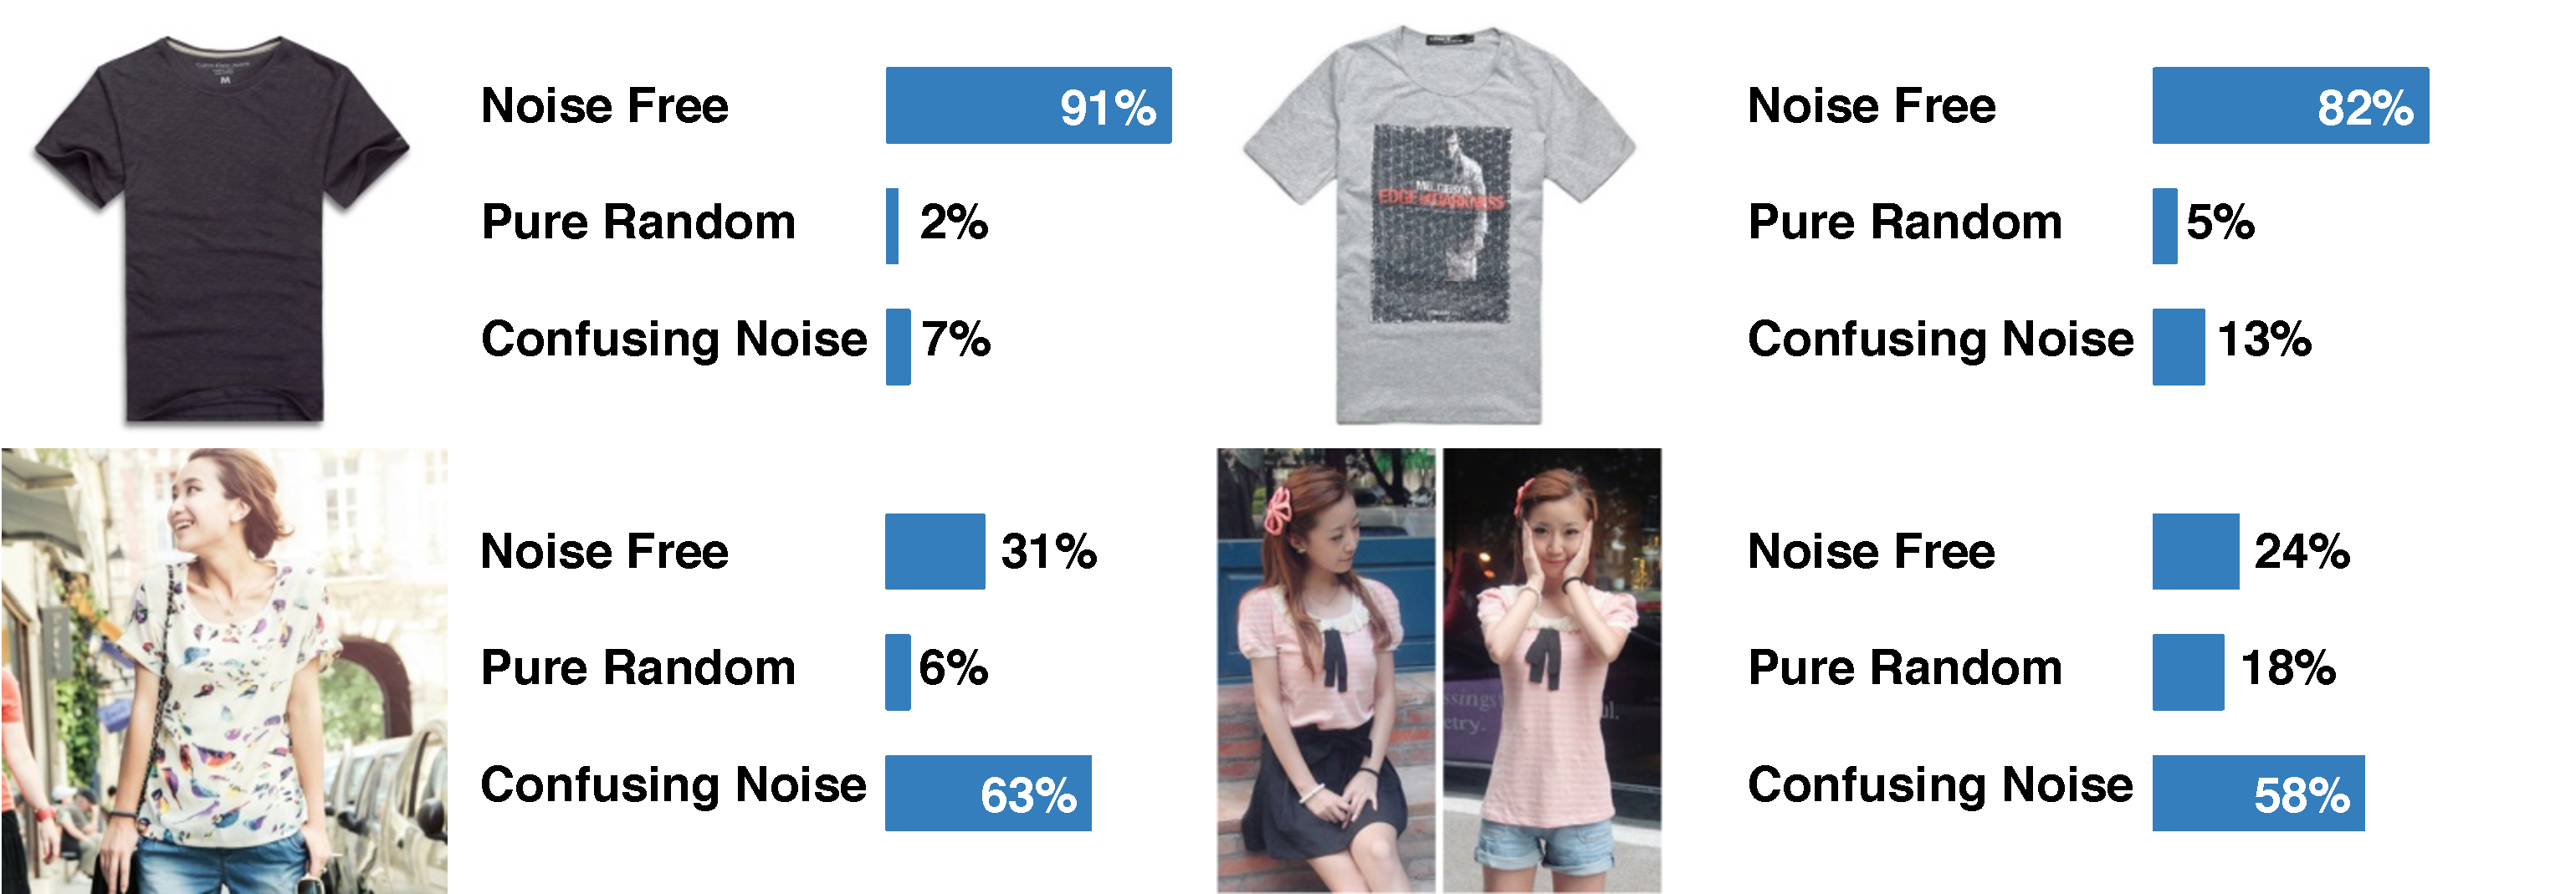
\includegraphics[width=1.0\linewidth]{figure/noise_level.pdf}
\end{center}
\caption{Predicting noise types of four different ``T-shirt'' images. The top two can be recognized with little ambiguity, while the bottom two are easily confusing with the class ``Chiffon''. Image content can affect the possibility of it to be mislabeled.}
\label{fig:compare_noise_level}
\end{figure}

To illustrate the relations between noisy and true labels, we derive their conditional probability from Eq~\ref{eq:joint_distribution}
\begin{equation}
    p(\tilde{\vec{y}} | \vec{y}, \vec{x}) = \sum_{\vec{z}} p(\tilde{\vec{y}}, \vec{z} | \vec{y}, \vec{x}) = \sum_{\vec{z}} p(\tilde{\vec{y}} | \vec{y}, \vec{z}) p(\vec{z} | \vec{x})
\end{equation}
which can be interpreted as a mixture model. Given an input image $\vec{x}$, the conditional probability $p(\vec{z} | \vec{x})$ can be seen as the prior of each mixture component. This makes a key difference between our work and~\cite{sukhbaatar2014learning}, where they assume $\tilde{\vec{y}}$ is conditionally independent with $\vec{x}$ if $\vec{y}$ is given. All the images share a same noise model in~\cite{sukhbaatar2014learning}, while in our approach each data sample has its own.

\subsection{Learning the Parameters} % (fold)
\label{sub:learning_the_parameters}
We exploit two CNNs to model $p(\vec{y} | \vec{x})$ and $p(\vec{z} | \vec{x})$ separately. Denote the parameter set of each CNN by $\theta_1$ and $\theta_2$. Our goal is to find the optimal $\theta = \theta_1 \cup \theta_2$ that maximize the incomplete log-likelihood $\log p(\tilde{\vec{y}} | \vec{x}; \theta)$. The EM algorithm is used to iteratively solve this problem.

For any probability distribution $q(\vec{y}, \vec{z} | \tilde{\vec{y}}, \vec{x})$, we can derive a lower bound of the incomplete log-likelihood,
\begin{equation}
\begin{aligned}
    \log p(\tilde{\vec{y}} | \vec{x}; \theta) &= \log \sum_{\vec{y},\vec{z}} p(\tilde{\vec{y}}, \vec{y}, \vec{z} | \vec{x}; \theta) \\
    &\geq \sum_{\vec{y},\vec{z}} q(\vec{y}, \vec{z} | \tilde{\vec{y}}, \vec{x}) \log \frac{p(\tilde{\vec{y}}, \vec{y}, \vec{z} | \vec{x}; \theta)}{q(\vec{y}, \vec{z} | \tilde{\vec{y}}, \vec{x})}
\end{aligned}
\end{equation}
\textbf{E-Step} The difference between $\log p(\tilde{\vec{y}} | \vec{x}; \theta)$ and its lower bound is the Kullback-Leibler divergence $\mathrm{KL}\left(q(\vec{y}, \vec{z} | \tilde{\vec{y}}, \vec{x}) || p(\vec{y}, \vec{z} | \tilde{\vec{y}}, \vec{x}; \theta)\right)$, which is equal to zero if and only if $q(\vec{y}, \vec{z} | \tilde{\vec{y}}, \vec{x}) = p(\vec{y}, \vec{z} | \tilde{\vec{y}}, \vec{x}; \theta)$. Therefore, in each iteration $t$, we first compute the posterior of latent variables using the current parameters $\theta^{(t)}$:
\begin{multline} \label{eq:posterior}
    p(\vec{y}, \vec{z} | \tilde{\vec{y}}, \vec{x}; \theta^{(t)}) = \frac{p(\tilde{\vec{y}}, \vec{y}, \vec{z} | \vec{x}; \theta^{(t)})}{p(\tilde{\vec{y}} | \vec{x}; \theta^{(t)})} \\
    = \frac{p(\tilde{\vec{y}}|\vec{y},\vec{z};\theta^{(t)}) p(\vec{y}|\vec{x};\theta^{(t)}) p(\vec{z}|\vec{x};\theta^{(t)})}{\sum_{\vec{y}',\vec{z}'} p(\tilde{\vec{y}}|\vec{y}',\vec{z}';\theta^{(t)}) p(\vec{y}'|\vec{x};\theta^{(t)}) p(\vec{z}'|\vec{x};\theta^{(t)})}
\end{multline}
Then the expected complete log-likelihood can be written as
\begin{equation}
    Q(\theta; \theta^{(t)}) = \sum_{\vec{y},\vec{z}} p(\vec{y}, \vec{z} | \tilde{\vec{y}}, \vec{x}; \theta^{(t)}) \log p(\tilde{\vec{y}}, \vec{y}, \vec{z} | \vec{x}; \theta)
\end{equation}
\textbf{M-Step} We exploit two CNNs to model the probability $p(\vec{y}|\vec{x};\theta_1)$ and $p(\vec{z}|\vec{x};\theta_2)$, respectively. Thus the gradient of $Q$ \wrt $\theta$ can be decoupled into two parts:
\begin{multline} \label{eq:gradient}
    \frac{\partial Q}{\partial \theta} = \sum_{\vec{y},\vec{z}} p(\vec{y}, \vec{z} | \tilde{\vec{y}}, \vec{x}; \theta^{(t)}) \frac{\partial}{\partial \theta} \log p(\tilde{\vec{y}}, \vec{y}, \vec{z} | \vec{x}; \theta) \\
    = \sum_{\vec{y}} p(\vec{y} | \tilde{\vec{y}}, \vec{x}; \theta^{(t)}) \frac{\partial}{\partial \theta_1} \log p(\vec{y}|\vec{x};\theta_1) + \\
      \sum_{\vec{z}} p(\vec{z} | \tilde{\vec{y}}, \vec{x}; \theta^{(t)}) \frac{\partial}{\partial \theta_2} \log p(\vec{z}|\vec{x};\theta_2)
\end{multline}

The M-Step above is equivalent to minimizing the cross entropy between the estimated ground truth distribution and the prediction of the classifier.
% subsection learning_the_parameters (end)

\subsection{Estimating Matrix $\mat{C}$} % (fold)
\label{sub:confusion_estimation}
Notice that we do not set parameters to the conditional probability $p(\tilde{\vec{y}}|\vec{y},\vec{z})$ in Eq~\eqref{eq:likelihood} and keep it unchanged during the learning process. Because without other regularizations, learning all the three parts in Eq~\eqref{eq:joint_distribution} could lead to trivial solutions. For example, the network will always predict $\vec{y}_1 = 1$, $\vec{z}_3 = 1$, and the matrix $\mat{C}$ is learned to make $\mat{C}_{1i} = 1$ for all $i$. To avoid such degeneration, we estimate $\mat{C}$ on a relatively small dataset $\mathcal{D}_c = \{(\vec{x},\vec{y},\tilde{\vec{y}})\}_N$, where we have $N$ images with both clean and noisy labels. As prior information about $\vec{z}$ is not available, we solve the following optimization problem:
\begin{equation} \label{eq:opt_all}
    \max_{\mat{C},\vec{z}^{(1)},\cdots,\vec{z}^{(N)}} \sum_{i=1}^N \log p(\tilde{\vec{y}}^{(i)}|\vec{y}^{(i)},\vec{z}^{(i)})
\end{equation}
Obviously, sample $i$ contributes nothing to the optimal $\mat{C}^*$ if $\vec{y}^{(i)}$ and $\tilde{\vec{y}}^{(i)}$ are equal. So that we discard those samples and reinterpret the problem in another form by exploiting Eq~\ref{eq:likelihood}:
\begin{equation}
\begin{aligned}
\max_{\mat{C},\vec{t}} \quad & E=\sum_{i=1}^{N'} \log \alpha^{\vec{t}_i} + \log (\tilde{\vec{y}}^{(i)T} \mat{C} \vec{y}^{(i)})^{1-\vec{t}_i}\\
\text{subject to} \quad & \mat{C} \text{ is a stochastic matrix of size } L\times L \\
                    & \vec{t} \in \{0,1\}^{N'}
\end{aligned}
\end{equation}
where $\alpha=\frac{1}{L-1}$ and $N'$ is the number of remaining samples. The semantic meaning of the above formulation is that we need to assign each $(\vec{y},\tilde{\vec{y}})$ pair the optimal noise type, while finding the optimal $\mat{C}$ simultaneously.

Next, we will show that the problem can be solved by a simple yet efficient algorithm in $O(N'+L^2)$ time complexity. Denote the optimal solution by $\mat{C}^*$ and $\vec{t}^*$
\begin{theorem}
$\mat{C}^*_{ij} \neq 0 \Rightarrow \mat{C}^*_{ij} > \alpha, \forall i,j \in \{1,\dots,L\}$
\end{theorem}
\begin{proof}
Suppose there exists some $i,j$ such that $0 < \mat{C}^*_{ij} \leq \alpha$. Then we conduct the following operations. First, we set $\mat{C}^*_{ij}=0$ while adding its original value to other elements in column $j$. Second, for all the samples $n$ where $\tilde{\vec{y}}^{(n)}_i=1$ and $\vec{y}^{(n)}_j=1$, we set $\vec{t}_n$ to 1. The resulting $E$ will get increased, which leads to a contradiction.
\end{proof}
\begin{theorem}
$(\tilde{\vec{y}}^{(i)},\vec{y}^{(i)})=(\tilde{\vec{y}}^{(j)},\vec{y}^{(j)}) \Rightarrow \vec{t}^*_i=\vec{t}^*_j, \forall i,j \in \{1,\dots,N'\}$
\end{theorem}
\begin{proof}
Suppose $\tilde{\vec{y}}^{(i)}_k=\tilde{\vec{y}}^{(j)}_k=1$ and $\vec{y}^{(i)}_l=\vec{y}^{(j)}_l=1$ but $\vec{t}^*_i \neq \vec{t}^*_j$. From Theorem 1 we know that elements in $\mat{C}^*$ is either 0 or greater than $\alpha$. If $\mat{C}^*_{kl}=0$, we can set $\vec{t}^*_i=\vec{t}^*_j=1$, otherwise we can set $\vec{t}^*_i=\vec{t}^*_j=0$. In either case the resulting $E$ will get increased, which leads to a contradiction.
\end{proof}
\begin{theorem}
$\tilde{\vec{y}}^{(i)T} \mat{C}^* \vec{y}^{(i)} > \alpha \Leftrightarrow \vec{t}^*_i=0$ and $\tilde{\vec{y}}^{(i)T} \mat{C}^* \vec{y}^{(i)} = 0 \Leftrightarrow \vec{t}^*_i=1, \forall i \in \{1,\dots,N'\}$
\end{theorem}
\begin{proof}
The first part is straightforward. For the second part, $\vec{t}^*_i=1$ implies $\tilde{\vec{y}}^{(i)T} \mat{C}^* \vec{y}^{(i)} \leq \alpha$. By using Theorem 1 we know that $\tilde{\vec{y}}^{(i)T} \mat{C}^* \vec{y}^{(i)} = 0$.
\end{proof}

Notice that if the true label is class $i$ while the noisy label is class $j$, then it can only affect the value of $\mat{C}_{ij}$. Thus each column of $\mat{C}$ can be optimized separately. Theorem 1 further shows that samples with same pair of $(\tilde{\vec{y}},\vec{y})$ share a same noise type. Then what really matters is the frequencies of all the $L\times L$ pairs of $(\tilde{\vec{y}},\vec{y})$. Considering a particular column $\vec{c}$, suppose there are $M$ samples affecting this column. We can count the frequencies of noisy label class 1 to $L$ as $m_1,\dots,m_L$ and might as well assume $m_1\geq m_2\geq \cdots \geq m_L$. The problem is then converted to
\begin{equation}
\begin{aligned}
\max_{\vec{c},\vec{t}} \quad & E=\sum_{k=1}^{L} m_k \left(\log \alpha^{\vec{t}_k} + \log \mat{c}_k^{1-\vec{t}_k}\right),\\
\text{subject to} \quad & \vec{c} \in [0,1]^L, \sum_{k=1}^{L} \vec{c}_k = 1,\\
                    & \vec{t} \in \{0,1\}^{L}.
\end{aligned}
\end{equation}

Due to the rearrangement inequality, we can prove that in the optimal solution,
\begin{equation}
    \max(\alpha,\vec{c}^*_1) \geq \max(\alpha,\vec{c}^*_2) \geq \cdots \geq \max(\alpha,\vec{c}^*_L).
\end{equation}
Then by using Theorem 3, there must exist a $k^* \in \{1,\dots,L\}$ such that
\begin{equation} \label{eq:opt_t}
\begin{aligned}
    &\vec{t}^*_i = 0, i = 1,\dots,k^* \\
    &\vec{t}^*_i = 1, i = k^*+1,\dots,L.
\end{aligned}
\end{equation}
This also implies that only the first $k^*$ elements of $\vec{c}^*$ have nonzero values (greater than $\alpha$ actually). Furthermore, if $k^*$ is known, finding the optimal $\vec{c}^*$ is to solve the following problem:
\begin{equation}
\begin{aligned}
\max_{\vec{c}} \quad & E=\sum_{k=1}^{k^*} m_k \log \mat{c}_k,\\
\text{subject to} \quad & \vec{c} \in [0,1]^L, \sum_{k=1}^{k^*} \vec{c}_k = 1,
\end{aligned}
\end{equation}
whose solution is
\begin{equation} \label{eq:opt_c}
\begin{aligned}
    &\vec{c}^*_i = \frac{m_i}{\sum_{k=1}^{k^*}{m_k}}, i = 1,\dots,k^*,\\
    &\vec{c}^*_i = 0, i = k^*+1,\dots,L.
\end{aligned}
\end{equation}

The above analysis leads to a simple algorithm. We enumerate $k^*$ from 1 to $L$. For each $k^*$, $\vec{t}^*$ and $\vec{c}^*$ are computed by using Eq~\eqref{eq:opt_t} and~\eqref{eq:opt_c}, respectively. Then we evaluate the objective function $E$ and record the best solution.


% subsection confusion_estimation (end)

% section label_noise_model (end)

\section{Deep Learning from Noisy Labels} % (fold)
\label{sec:deep_learning_from_noisy_labels}

\begin{figure*}
\begin{center}
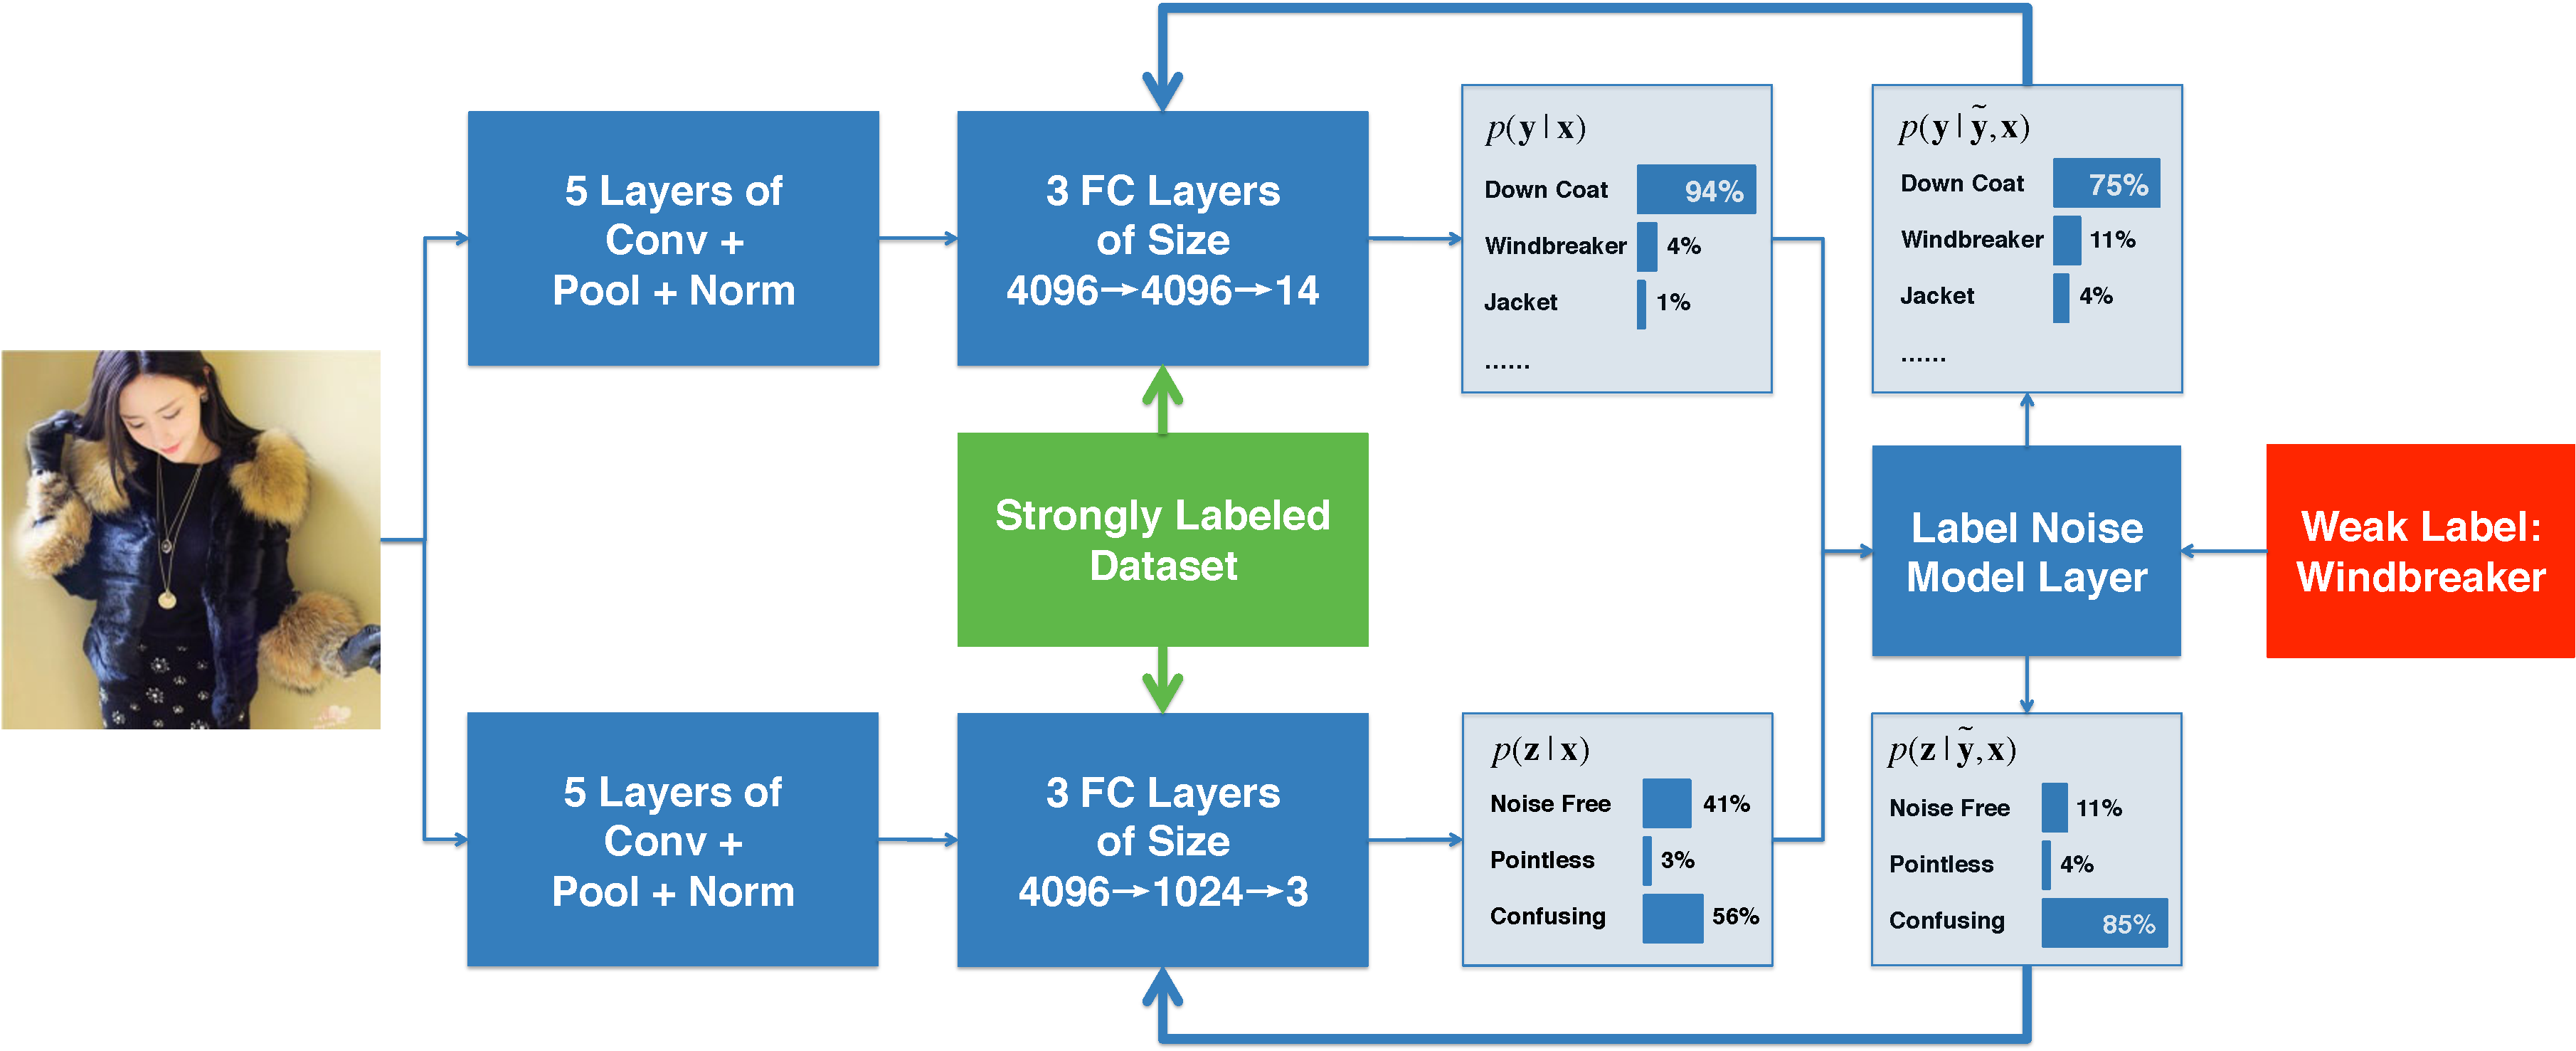
\includegraphics[width=0.9\linewidth]{figure/diagram.pdf}
\end{center}
\caption{System diagram of our method. Two CNNs are used to predict the class label $p(\vec{y}|\vec{x})$ and the noise type $p(\vec{z}|\vec{x})$, respectively. The label noise model layer infers the true label according to the predictions and the noisy label, which is then used to supervise the training of CNNs. Data with clean labels are also mixed in to prevent the models from drifting away.}
\label{fig:framework}
\end{figure*}

We integrate the proposed label noise model into a deep learning framework. As demonstrated in Figure~\ref{fig:framework}, we predict the probability $p(\vec{y}|\vec{x})$ and $p(\vec{z}|\vec{x})$ by using two independent CNNs. Moreover, we append a label noise model layer at the end, which takes as input the CNNs' prediction scores and the observed noisy label. Stochastic Gradient Ascent with backpropagation technique is used to approximately optimize the whole network. In each forward pass, the label noise model layer computes the posterior of latent variables according to Eq~\eqref{eq:posterior}. While in the backward pass, it computes the gradients according to Eq~\eqref{eq:gradient}.

% The forward procedure is summarized in Algorithm~\ref{alg:forward}, and the backward pass for computing gradient with respect to $p(\vec{y}|\vec{x})$ is illustrated in Algorithm~\ref{alg:backward}.

% \begin{algorithm}
%     \SetKwData{Sum}{sum}
%     \SetKwFunction{Softmax}{Softmax}\SetKwFunction{Q}{Q}
%     \SetKwInOut{Input}{input}\SetKwInOut{Output}{output}

%     \Input{Observed weak label vector $\tilde{\vec{y}}$ of size $N$}
%     \Input{Object class scores matrix $Y$ of size $N \times L$}
%     \Input{Noise type scores matrix $Z$ of size $N \times 3$}
%     \Output{Posterior probability matrix $P$ of size $L \times 3$}
%     \BlankLine

%     $P_y \leftarrow$ \Softmax{$Y$}\;
%     $P_z \leftarrow$ \Softmax{$Z$}\;
%     \BlankLine

%     \emph{\Q is the function that implements Eq~\eqref{eq:likelihood}}\;
%     \BlankLine

%     \For {$i \leftarrow 1$ \KwTo $N$} {
%         \Sum $\leftarrow 0$\;
%         \For {$j \leftarrow 1$ \KwTo $L$} {
%             \For {$k \leftarrow 1$ \KwTo $3$} {
%                 $P[i,j,k] \leftarrow P_y[i,j] \times P_z[i,k] \times$ \Q{$\tilde{\vec{y}}$,j,k}\;
%                 \Sum $\leftarrow$ \Sum$+ P[i,j,k]$\;
%             }
%         }
%         $P[i,:,:] \leftarrow P[i,:,:] /$ \Sum\;
%     }

%     \caption{Forward pass}
%     \label{alg:forward}
% \end{algorithm}
% \begin{algorithm}
%     \SetKwData{Sum}{sum}
%     \SetKwInOut{Input}{input}\SetKwInOut{Output}{output}

%     \Input{Object class scores matrix $Y$ of size $N \times L$}
%     \Input{Posterior probability matrix $P$ of size $L \times 3$}
%     \Output{Gradient matrix $\Delta_Y$ of size $N \times L$}
%     \BlankLine

%     \For {$i \leftarrow 1$ \KwTo $N$} {
%         \For {$j \leftarrow 1$ \KwTo $L$} {
%             \Sum $\leftarrow 0$\;
%             \For {$k \leftarrow 1$ \KwTo $3$} {
%                 \Sum $\leftarrow$ \Sum$+ P[i,j,k]$\;
%             }
%             $\Delta_Y[i,:] \leftarrow \Delta_Y[i,:] + $ \Sum $\times Y[i,:]$\;
%             $\Delta_Y[i,j] \leftarrow \Delta_Y[i,j] - $ \Sum\;
%         }
%     }


%     \caption{Backward pass for computing gradient w.r.t. object class scores}
%     \label{alg:backward}
% \end{algorithm}

Directly training the whole network with random initialization is impractical, because the posterior computation could be totally wrong. Therefore, we need to pretrain each CNN component with strongly supervised data. Images and their ground truth labels in the dataset $\mathcal{D}_c$ are used to train the CNN that predicts $p(\vec{y}|\vec{x})$. On the other hand, the optimal solutions of $\vec{z}^{(1)},\cdots,\vec{z}^{(N)}$ in Eq~\eqref{eq:opt_all} are used to train the CNN that predicts $p(\vec{z}|\vec{x})$.

After both CNN components are properly pretrained, we can start to train the whole network with massive noisy labeled data. However, some practical issues need to be further discussed. First, if we merely use noisy labels, we will lose precious knowledge that we have gained before and the model could be drifted. Therefore, we need to mix the data with clean labels into our training set, which is depicted in Figure~\ref{fig:framework} as the extra supervisions for the two CNNs. Then each CNN receives two kinds of gradients, one is from the clean labels and the other is from the noisy labels. We denote them by $\Delta_c$ and $\Delta_n$, respectively. A potential problem is that $|\Delta_c| \ll |\Delta_n|$, because clean data is much less than noisy data. To deal with this problem, we bootstrap the clean data $\mathcal{D}_c$ to half amount of the noisy data $\mathcal{D}_{\eta}$. This upsampling process brings another advantage --- the gradients we calculated in each mini-batch are much more stable.

Our proposed method has the ability to figure out the true label given the image and its noisy label. From the perspective of information, our model predicts from two kinds of clues: what are the true labels for other similar images; and how easily for the image to be mislabeled. Label Propagation method~\cite{zhu2002learning} explicitly uses the first kind of information, while we implicitly capture it with a discriminative deep model. On the other hand, the second kind of information correlates the image content with the label noise, which can help distinguish between hard samples and mislabeled ones.
% section deep_learning_from_noisy_labels (end)

\section{Experiments} % (fold)
\label{sec:experiments}

\subsection{Dataset} % (fold)
\label{sub:dataset}
Since there is no publicly available dataset that has both clean and noisy labels, to test our method under real-world scenario, we build a large-scale clothing dataset by crawling images from several online shopping websites. More than a million images are collected together with their surrounding texts provided by the sellers. These surrounding texts usually contain rich information about the products, which can be further converted to visual tags. Specific to our task of clothing classification, we define $14$ class labels: T-shirt, Shirt, Knitwear, Chiffon, Sweater, Hoodie, Windbreaker, Jacket, Down Coat, Suit, Shawl, Dress, Vest, and Underwear. We assign an image a noisy label if we find its surrounding text contains only the keywords of that label, otherwise we discard the image to reduce ambiguity.

After that we manually refine the noisy labels of a small portion of all the images and split them into training ($\mathcal{D}_c$), validation and test sets. On the other hand, the remaining samples construct the noisy labeled training dataset ($\mathcal{D}_{\eta}$). A crucial step here is to remove from $\mathcal{D}_c$ and $\mathcal{D}_{\eta}$ the images that are near duplicate with any image in the validation or test set, which ensures the reliability of our test protocol. Finally, the size of training datasets are $|\mathcal{D}_c| = 47,570$ and $|\mathcal{D}_{\eta}| = 10^6$, while validation and test set have $14,313$ and $10,526$ images, respectively.

The confusion matrix between clean and noisy labels is presented in Figure~\ref{fig:cm_strong_weak}. We can see that the overall accuracy is $61.54\%$, and some pairs of classes are very confusing with each other (\eg Knitwear and Sweater), which means that the noisy labels are not so reliable.

\begin{figure}[t]
\begin{center}
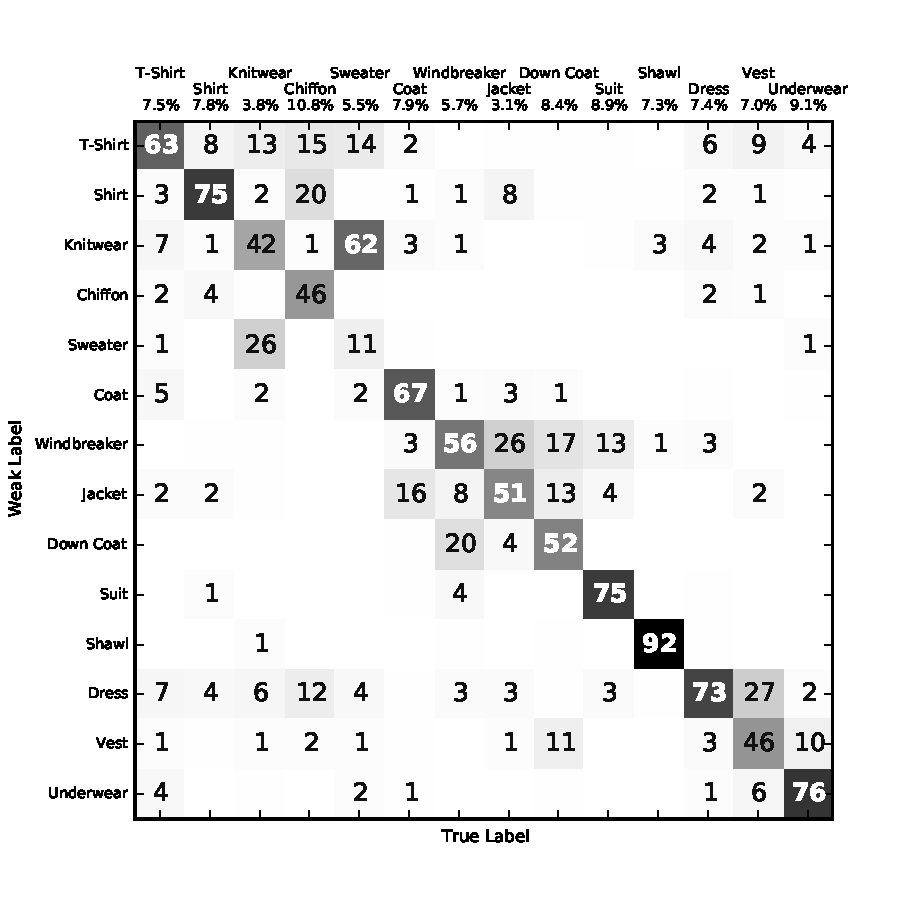
\includegraphics[width=1.0\linewidth]{figure/cm_strong_weak_labels.pdf}
\end{center}
\caption{Confusion matrix between clean and noisy labels. We hide extremely small grid numbers for better demonstration. Frequency of each true label is listed at the top of each column. The overall accuracy is $61.54\%$, which indicates that the noisy labels are not reliable.}
\label{fig:cm_strong_weak}
\end{figure}
% subsection dataset (end)

\subsection{Evaluation on the Collected Dataset} % (fold)
\label{sub:evaluation}
We validate our method through a series of experiments conducted on the collected dataset. Our implementation is based on Caffe~\cite{jia2014caffe}, and the \texttt{bvlc\_reference\_caffenet}\footnote{\url{http://caffe.berkeleyvision.org/model_zoo.html}} is chosen as the baseline model, which approximates AlexNet~\cite{krizhevsky2012imagenet}. Besides, we reimplement two other approaches. One is a semi-supervised learning method called Pseudo-Label~\cite{lee2013pseudo}, which exploits classifier's prediction as ground truth for unlabeled data. The other one is the Bottom-Up method introduced in~\cite{sukhbaatar2014learning}, where the relation between noisy labels and clean labels are built by a confusion matrix $Q$. In the experiments, we directly use the true $Q$ as shown in Figure~\ref{fig:cm_strong_weak} instead of estimating its values.

We list all the experiment settings in Table~\ref{tab:exp}. Different methods require different training data. We use only the clean data $\mathcal{D}_c$ to get the baselines under strong supervisions. On the other hand, when all the data are used, we upsample the clean data as discussed in Section~\ref{sec:deep_learning_from_noisy_labels}. Meanwhile, the noisy labels of $\mathcal{D}_{\eta}$ are treated as true labels for AlexNet, and are discarded for Pseudo-Label.

In general, we use a mini-batch size of $256$. The learning rate is initialized to be $0.001$ and is divided by $10$ after every $50,000$ iterations. We keep training each model until convergence. Classification accuracies on the test set are presented in Table~\ref{tab:exp}.

\begin{table*}[t]
\begin{center}
\begin{tabular}{c|c|c|c|c}
\hline
\# & Method & Training Data & Initialization & Test Accuracy\\
\hline\hline
1 & AlexNet & $\mathcal{D}_c$ & random & 64.54\% \\
2 & AlexNet & $\mathcal{D}_c$ & ImageNet pretrained & 72.63\% \\
3 & AlexNet & upsampled $\mathcal{D}_c$ and $\mathcal{D}_{\eta}$ as ground truths & random & 74.03\% \\
4 & AlexNet & upsampled $\mathcal{D}_c$ and $\mathcal{D}_{\eta}$ as ground truths & ImaegNet pretrained & 75.13\% \\
5 & AlexNet & upsampled $\mathcal{D}_c$ and $\mathcal{D}_{\eta}$ as ground truths & model \#2 & 75.30\% \\
6 & Pseudo-Label\cite{lee2013pseudo} & upsampled $\mathcal{D}_c$ and $\mathcal{D}_{\eta}$ as unlabeled & model \#2 & 73.04\% \\
7 & Bottom-Up~\cite{sukhbaatar2014learning} & $\mathcal{D}_c$ and $\mathcal{D}_{\eta}$ & model \#2 & 76.22\% \\
8 & Ours & $\mathcal{D}_c$ and $\mathcal{D}_{\eta}$ & model \#2 & \textbf{78.24\%} \\
\hline
\end{tabular}
\end{center}
\caption{Experiment results on the collected dataset}
\label{tab:exp}
\end{table*}

% \begin{table}
% \begin{center}
% \begin{tabular}{c|c|c}
% \hline
% \# & Validation Accuracy & Test Accuracy \\
% \hline\hline
% 1 & 64.28\% & 64.54\% \\
% \hline
% 2 & 72.21\% & 72.63\% \\
% \hline
% 3 & 73.76\% & 74.03\% \\
% \hline
% 4 & 75.06\% & 75.13\% \\
% \hline
% 5 & 75.57\% & 75.30\% \\
% \hline
% 6 & 73.10\% & 73.04\% \\
% \hline
% 7 & 75.97\% & 76.22\% \\
% \hline
% 8 & \textbf{77.65\%} & \textbf{78.24\%} \\
% \hline
% \end{tabular}
% \end{center}
% \caption{Classification accuracies on validation and test set}
% \label{tab:accuracy}
% \end{table}

\begin{figure*}
\begin{center}
\end{center}
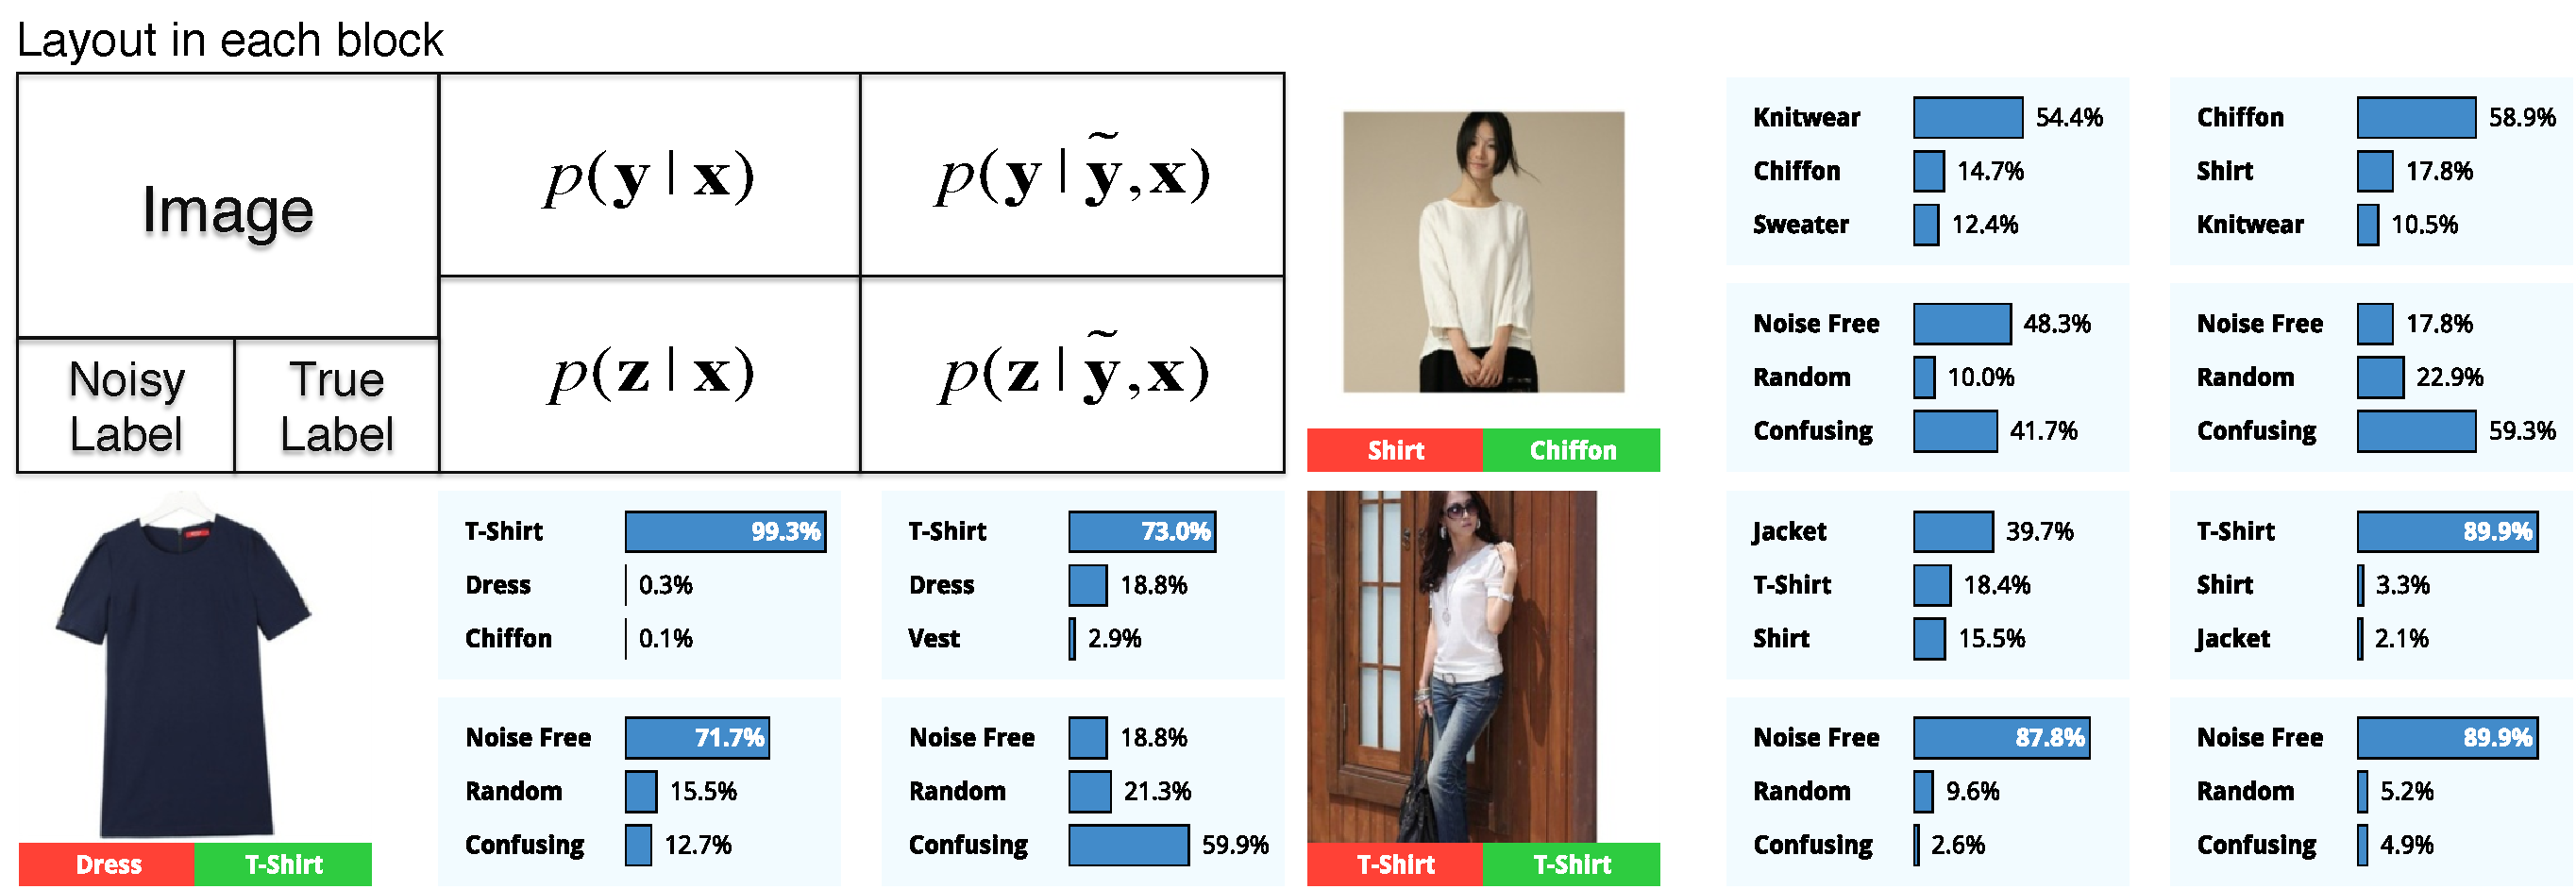
\includegraphics[width=1.0\linewidth]{figure/model_output.pdf}
\caption{Examples of handling noisy labels. The information layout in each block is illustrated in the top-left one.}
\label{fig:model_output}
\end{figure*}

We first study the effect of transfer learning and massive noisy labeled data. From row \#1 we can see that training a CNN from scratch with only small amount of clean data can result in bad performance. To deal with this problem, finetuning from an ImageNet pretrained model can significantly improve the accuracy, as shown in row \#2. However, by comparing row \#2 and \#3, we find that training with random initialization on additional massive noisy labeled data is better than finetuning only on the clean data, which demonstrates the power of using large-scale yet easily obtained noisy labeled data. The accuracy can be further improved if we finetune the model either from an ImageNet pretrained one or model \#2. The latter one has slightly better performance thus is used to initialize the remaining methods.

Next, from row \#6 we can see that semi-supervised learning methods may not be a good choice when massive noisy labeled data are available. Although model \#6 achieves marginally better result than its base model, it is significantly inferior to model \#5, which indicates that simply discarding all the noisy labels cannot make the full use of these information.

Finally, row \#7 and \#8 show the effect of modeling the label noise. Model \#7 is only $0.9\%$ better than the baseline model \#5, while our method gains improvement of $2.9\%$. This result does credit to our image dependent label noise model, which fits better to the noisy labeled data crawled from the Internet.

\subsection{Evaluation on Synthetic Dataset} % (fold)
\label{sub:evaluation_on_synthetic_dataset}
We also conduct synthetic experiments on CIFAR-10 following the settings of~\cite{sukhbaatar2014learning}. We first randomly generate a confusion matrix $Q$ between clean labels and noisy labels, and then corrupt the training labels according to it. Based on Caffe's CIFAR10-quick model, we compare~\cite{sukhbaatar2014learning} (Bottom Up with true $Q$) with our model under different noise levels. The test accuracies are reported in Table~\ref{tab:accuracy_synthetic}.

\begin{table}
\begin{center}
\begin{tabular}{c|c|c|c}
\hline
Noise Level & Base Model & \cite{sukhbaatar2014learning} & Ours \\
\hline\hline
30\% & 65.57\% & 69.73\% & 69.81\% \\
\hline
40\% & 62.38\% & 66.66\% & 66.76\% \\
\hline
50\% & 57.36\% & 63.39\% & 63.00\% \\
\hline
\end{tabular}
\end{center}
\caption{Accuracies on CIFAR-10 with synthetic label noise}
\label{tab:accuracy_synthetic}
\end{table}

It should be noticed that~\cite{sukhbaatar2014learning} assumed the distribution of noisy labels only depends on classes, while we assume it also depends on image content. This kind of synthetic label noise exactly matches their assumption but is unfavored to our model. Thus the noise type predictions in our model could be less informative. Nevertheless, our model achieves comparable results with~\cite{sukhbaatar2014learning}.
% subsection evaluation_on_synthetic_dataset (end)


\subsection{Effect of Noise Estimation} % (fold)
\label{sub:effect_of_noise_estimation}
In order to understand how does our model handle noisy labels, we first show several examples in Figure~\ref{fig:model_output}. We can see that given a noisy label, our model exploits its current knowledge to estimate the probability distribution of the true label, and then use it as supervision instead of the noisy one. Another interesting observation is that if $p(\vec{y}|\vec{x})$ or $p(\vec{z}|\vec{x})$ goes wrong, our model can still figure out the correct label.

Next we demonstrate the effect of learning to predict the label noise type. We estimate $p(\vec{z}_2=1|\vec{x})+p(\vec{z}_3=1|\vec{x})$ on the validation set and sort the images accordingly in descending order. Then for each image, we check whether its noisy label mismatches its clean label. The rank-precision curve is plotted in Figure~\ref{fig:noise_prediction_rp}. It shows that the intuitive observation --- images tend to be mislabeled often share similar patterns --- is reasonable, and our model is trained to recognize such patterns to help handle noisy labels.

\begin{figure}[t]
\begin{center}
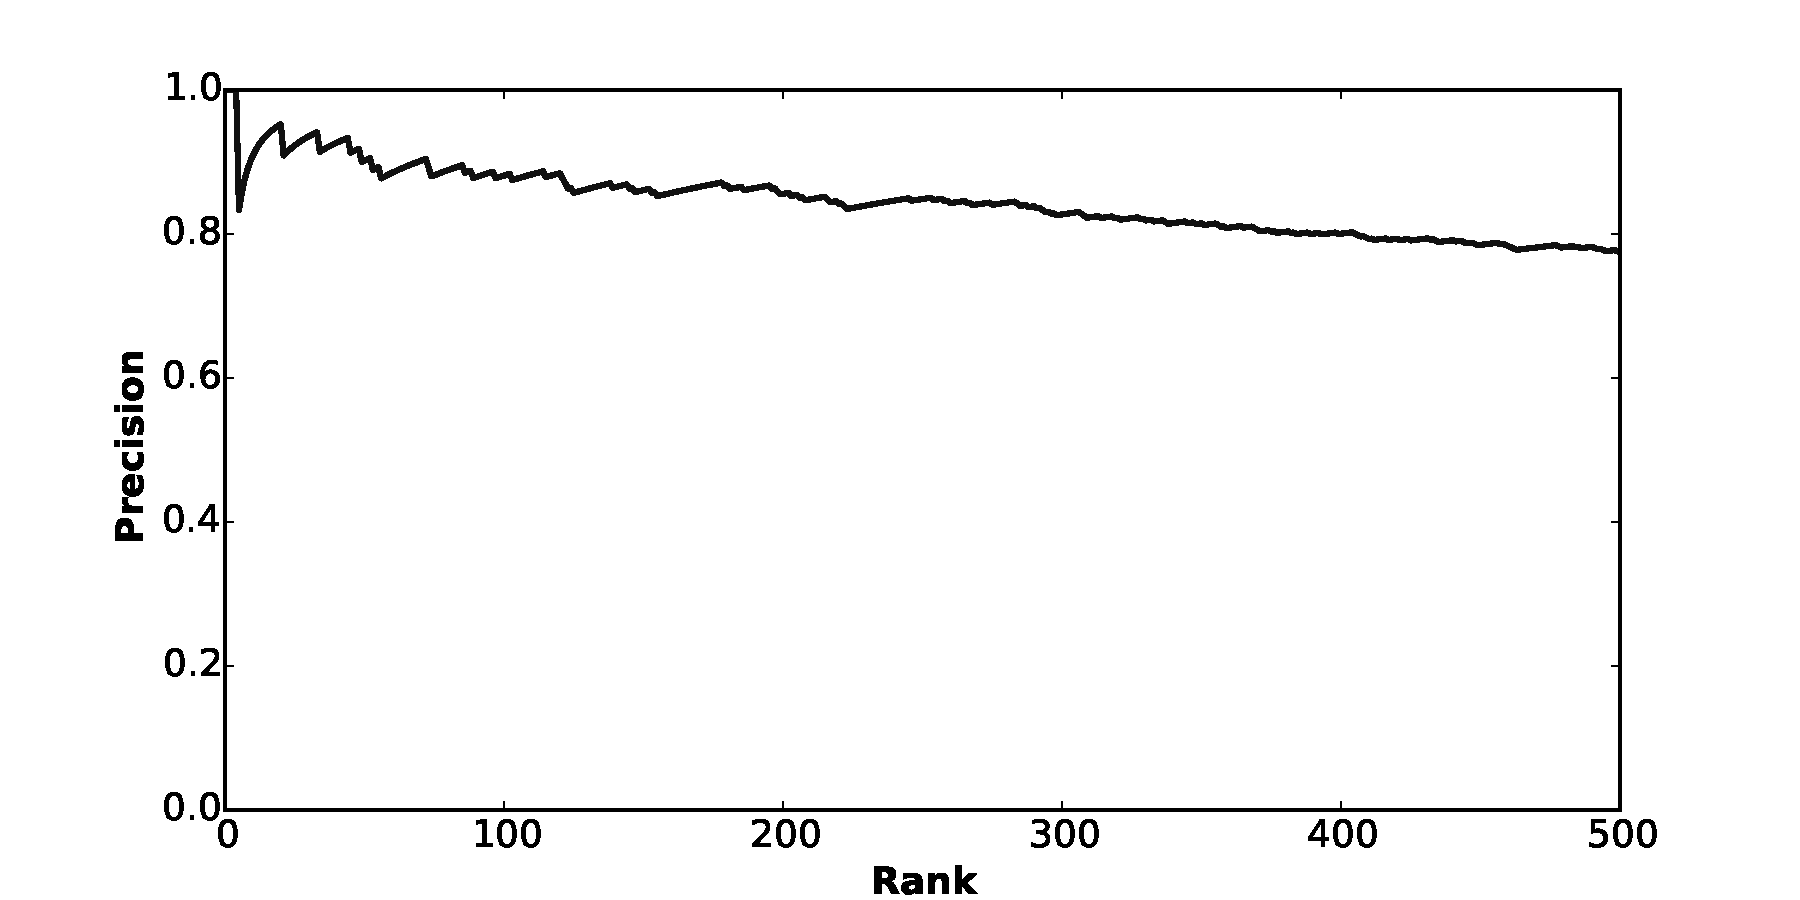
\includegraphics[width=1.0\linewidth]{figure/noise_prediction_rank_precision.pdf}
\end{center}
\caption{Rank-precision curve of label noise predictions}
\label{fig:noise_prediction_rp}
\end{figure}
% subsection effect_of_noise_estimation (end) 
% section experiments (end)

\section{Conclusion} % (fold)
\label{sec:conclusion}
In this paper, we raised the problem of training a classifier with limited clean annotations and massive noisy labeled data. We proposed a novel probabilistic model to describe how a noisy label is generated. Two latent variables --- true label and noise type --- were introduced to bridge the semantic gap between the observed image and its noisy label. We solved the problem by the EM algorithm and integrated it into a deep learning framework. Experiments on a collected large-scale clothing dataset showed that massive noisy label data could benefit the training of deep models, and utilizing our method could further improve the performance.
% section conclusion (end)

\section*{Acknowledgements}
\label{sec:acknowledgements}
This work is supported by the General Research Fund sponsored by the Research Grants Council of Hong Kong (Project Nos. CUHK14206114 and CUHK14207814) and the National Basic Research Program of China (973 program No. 2014CB340505).


{\small
\bibliographystyle{ieee}
\bibliography{references}
}

\end{document}
